\chapter{Fundamentação Teórica}
\addcontentsline{toc}{chapter}{Fundamentação Teórica}

Aprendizado de máquina é uma disciplina focada em duas questões interelacionadas: Como construir sistemas que automaticamente melhoram por meio da experiência? e quais as leis estatisticas,
computacionais e da teoria da informação que governam todos os sistemas de aprendizagem, incluindo computadores, seres humanos, e organizações?. O estudo de aprendizado de máquina é importante tanto
para responder a essas questões fundamentais de Engenharia e Ciência, quanto pelas aplicações computacionais que tem produzido \cite{Jordan}.
Um problema de aprendizado, pode ser colocado como um problema que reside em melhorar uma medida de performance, quando se executa alguma tarefa, através de algum tipo de experiência de treinamento \cite{Jordan}.

% Talvez mover esse bloco pra introdução
Para viabilizar o aprendizado de máquina, é necessário primeiramente entender os dados que serão utilizados no processo de aprendizado. Para entender esses dados
lançaremos mão de técnicas e conceitos estatísticos, que nos permitirão construir um modelo probabilístico que represente, por meio de uma função $f$, variáveis de entrada e de saída que compõe os dados com que estamos lidando. O fato de estarmos lidando com uma entrada e uma saída conhecida, nosso estudo irá se voltar para o \textit{aprendizado supervisionado}. Por outro lado, se no contexto do aprendizado, apenas dados de entrada estão disponíveis, é possível partir para o \textit{aprendizado não supervisionado}. 

Para o aprendizado supervionado, o conjunto de dados utilizado no treinamento será formado pelos dados em si, e pela saída esperada para esses dados\cite{Louridas}. Segundo \cite{James}, aprendizado estatístico supervisionado involve construir um modelo estatístico para prever ou estimar, uma saída a partir de uma ou mais entradas.


% Falar do alinhamento entre estatística e ciência da computação.

A disciplina de aprendizado de máquina pode ser subdividida da seguinte forma:
% TODO: Essa imagem tá muito pequena, aumentar a resolução.
\begin{figure}[h]
	\centering
	\label{fig01}
        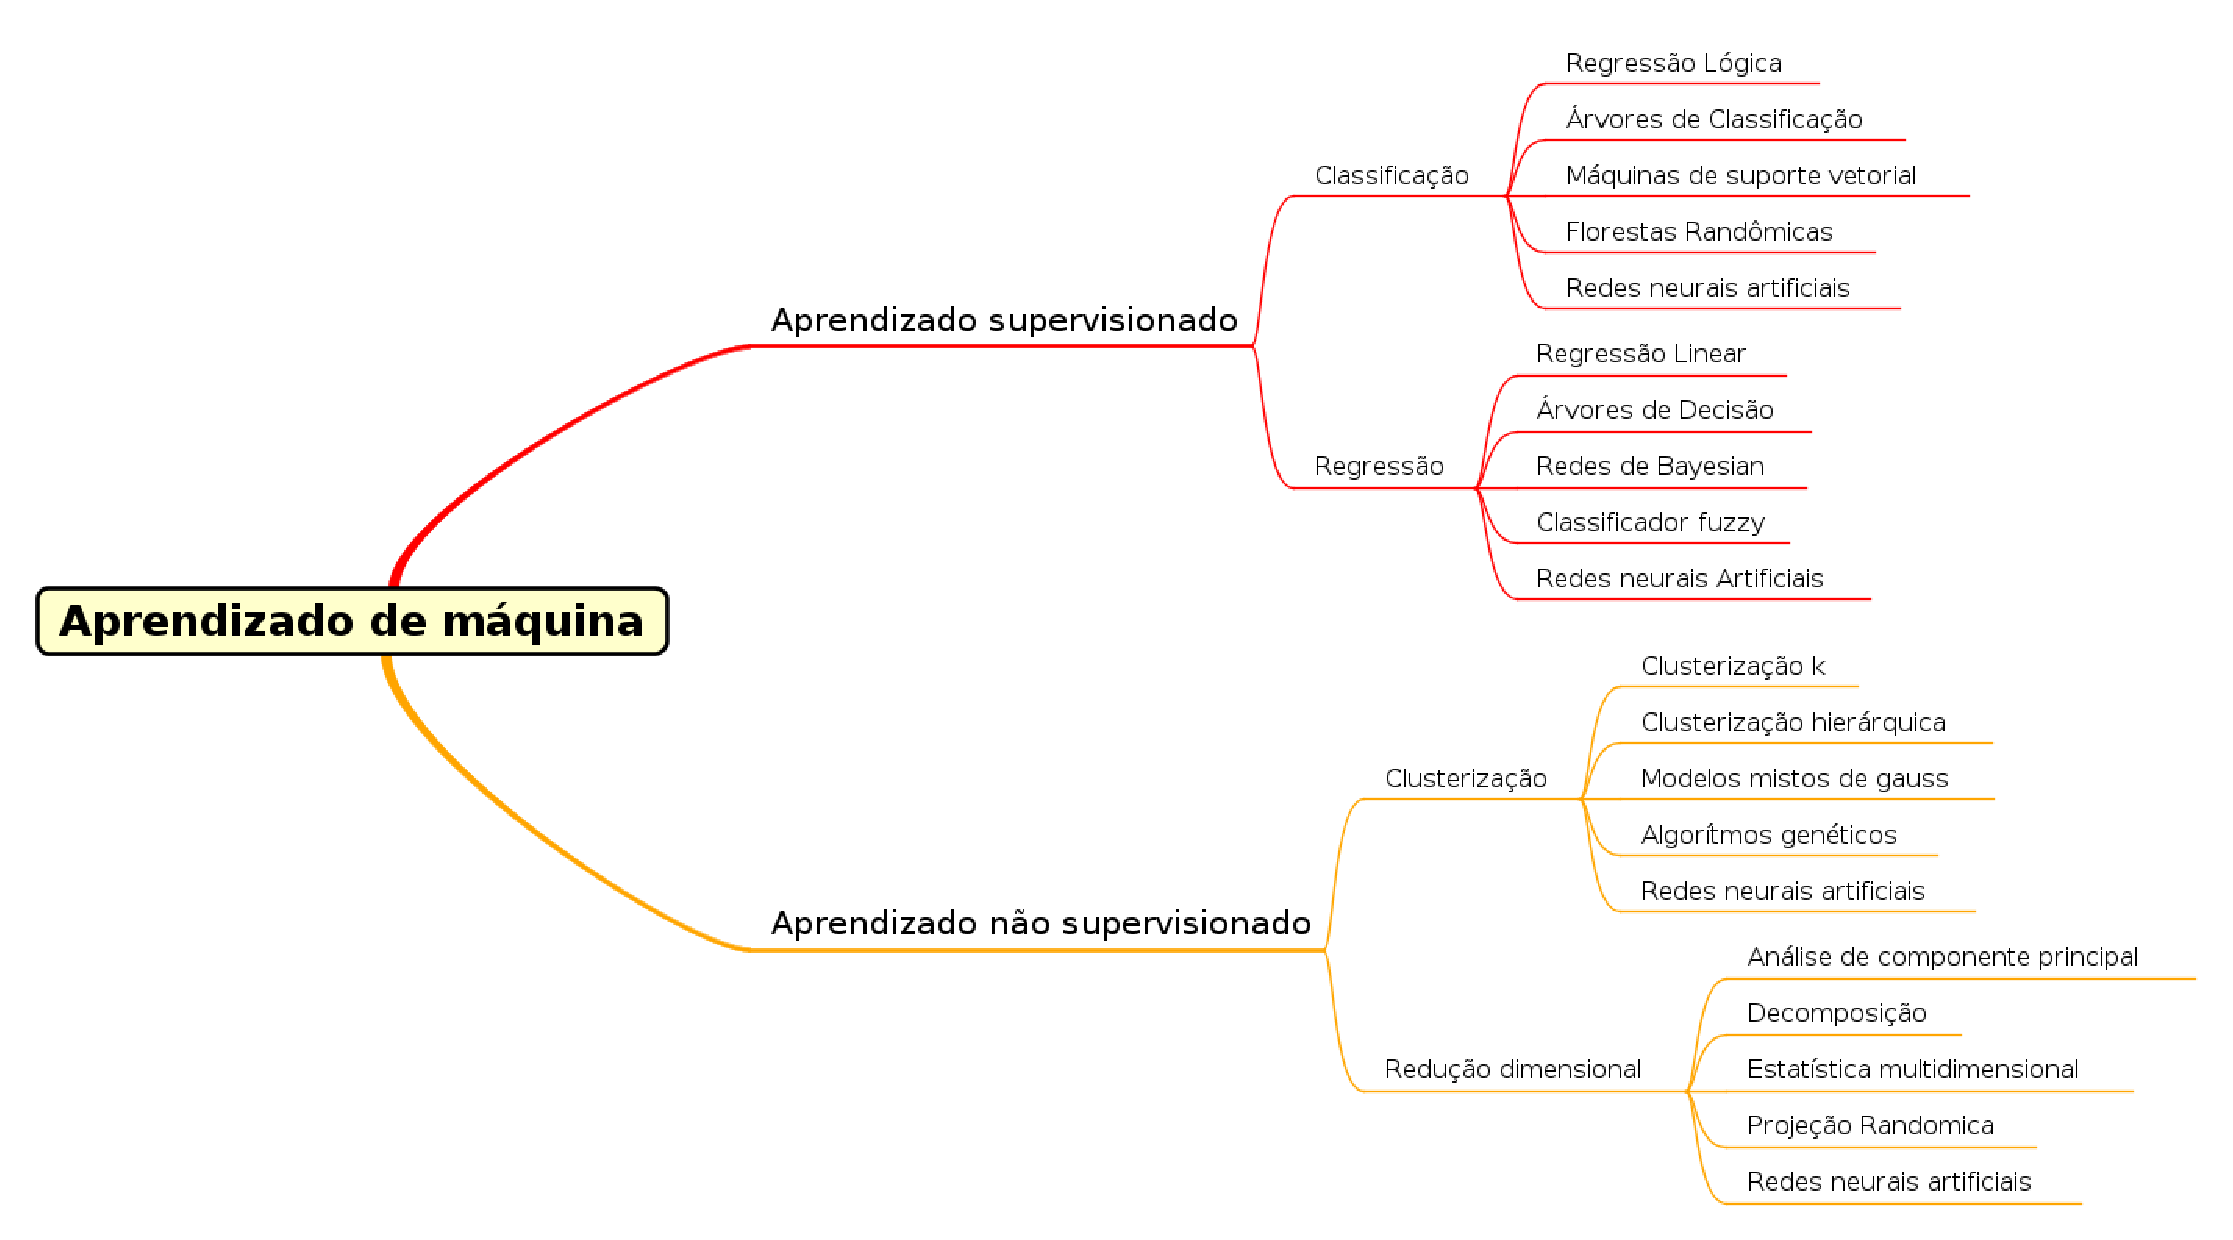
\includegraphics[scale=0.48]{figuras/mind1.eps}
	\caption{Abordagens para aprendizado de máquina}
\end{figure}
Neste capitulo iremos direcionar nossos estudos para o aprendizado supervisionado, pois eles são a base para o estudo de inferência.

\section{Aprendizado Estatístico}

Modelos probabilísticos, que representam uma distribuição probabilistica sobre variáveis randomicas, provê um conjuto de ferramentas sólidas e com princípios para
que problemas de incerteza possam ser resolvidos\cite{Sun}. Modelos probabilísticos podem ser lineares e não lineares. 

Modelos probabilisticos lineares descrevem uma variável dependente contínua, como uma função de uma ou mais variáveis independentes, possibilitando relacionar cada entrada à saída
esperada. Podemos definir então, que a entrada do nosso modelo probabilístico será um conjunto de dados representados aqui pelo simbolo $X$, e a nossa saída sendo representada pelo simbolo $Y$.  $X$ pode ser chamada de diversas formas, como preditor, variáveis independentes, características ou simplesmente variáveis.
O simbolo Y é normalmente chamado de resposta, ou variável dependente. Se consideramos um segundo exemplo dado por \cite{James}, em que o salário de um indivíduo é deduzido a partir
de fatores como a sua idade, escolaridade e o ano em que os dados foram coletados. Temos que $X = \{idade, escolaridade, ano\}$, enquanto Y representa o salário, ou seja, o fator que varia,
conforme $X_1(idade)$  ,$X_2(escolaridade)$ e $X_3(ano)$ variam.Poderiamos ter $p$ variáveis para $X$, nesse caso $p$ é igual a 3.
Podemos estabelecer também, que para cada $X_p$, teremos uma amostra de tamanho $n$. No exemplo dado por \cite{James},poderíamos ter uma amostra de tamanho $n$(vários valores de salário) para a váriável idependente $X_1$. Essa relação entre $p$ e $n$ nos permite estruturar esses dados matricialmente, aonde $X$ pode ser escrito como $p$x$n$\cite{James}.

$X$ pode ser definida como

\[
X_{i,j} = \begin{matrix}
x_{1,1} & x_{1,2} & \cdots & x_{1,j} \\
x_{2,1} & x_{2,2} & \cdots & x_{2,j} \\
\vdots  & \vdots  & \ddots & \vdots  \\
x_{i,1} & x_{i,2} & \cdots & x_{i,j} \\
\end{matrix}
\]

Sendo que cada coluna representa $p$ e cada linha representa $n$. Nesse contexto $x_i$ é um vetor de tamanho $p$, em que cada elemento do mesmo representa
um valor de $n$ atribuído a variável $p$ de posição $x_i$.

\[
X_{i} = \begin{matrix}
x_{i,1} \\
x_{i,2} \\
\vdots  \\
x_{i,3} \\
\end{matrix}
\]

Da  forma $x_j$ é um vetor de tamanho $n$, em que cada elemento representa uma valor da amostra de $n$ para uma variável $p$ específica.

\[
X_{j} = \begin{matrix}
x_{j,1} \\
x_{j,2} \\
\vdots  \\
x_{j,3} \\
\end{matrix}
\]

Podemos então representar essa relação entre $X$ e $Y$ da seguinte forma:

\[
  Y = f(X) + e
\]

$f$ é uma função fixa mas desconhecida de $X_1...X_p$, e $e$ é o termo de erro randomico, que é independente de $X$ e tem media zero. Essa formulação pode ser dita como ideal e teórica, uma vez que a função $f$ utilizada na prática, e o valor $Y$ encontrado como resultado, são estimativas, construidas a partir do aprendizado estatístico.
Podemos afirmar que $f$ representa a informação \textit{sistematica} que $X$ provê em releação a $Y$\cite{Jordan}.
Para definirmos $f$ devemos primeiro compreender a diferença entre inferência e predição.

\subsection{Predição}
Quando o objetivo do aprendizado reside em deduzir ou estimar um valor de $Y$, dado $X$, temos uma situação de predição. Podemos realizar essa predição utilizando
\[
  Y^* = f^*(X)
\]

$f^*$ é a estimativa para $f$, $Y^*$ é o valor previsto para $Y$. A precisão de $Y^*$ como uma previsão de $Y$ depende de dois valores, chamados de \textit{erro reduzivel} e \textit{erro irreduzivel}. No geral, $f^*$ não será uma estimativa perfeita de $f$, e essa imperfeição irá naturalmente, adicionar erros no resultado\cite{Jordan}.
O \textit{erro reduzivel} está relacionado ao erro de precisão de $f$. Ele é chamado de reduzível justamente pelo fato de que, por meio do treinamento, a precisão de $f^*$ pode ser cada vez melhor. Se uma amostra $n$ muito grande está disponível($n$ tende ao infinito) $f^*$ irá convergir para $f$\cite{Malhotra}. 
O erro \textit{erro irreduzivel} está relacionado ao erro $e$. Neste caso o erro independe de $X$, ou seja, não importa quão bom seja a nossa amostra de dados, muito menos o quão apropriada é a técnica de aprendizado estatístico utilizado, sempre haverá um erro $e$ que influência a precisão das previsões\cite{Jordan}.

A teoria de aprendizado estatístico tem por objetivo dar as condições necessárias e suficientes no que tange aos modelos estatísticos, que irá
garantir a consistência da estimativa de $f^*$, o que implica na convergência para $f$\cite{Malhotra}.

Aplicando a predição ao exemplo dado anteriormente do salário, poderíamos, estimando a função $f$, deduzir
o salário de um indivíduo a partir das variáveis de idade, escolaridade e ano de coleta dos dados. Abordagens não lineares
são comumente utilizadas para estimar $f$, quando se tem uma situação de predição.

\subsubsection{classificação}

Uma tarefa pode ser entendida como o processo de categorizar um dado, que será utilizado como entrada do algorítmo de aprendizado de máquina escolhido. Um bom exemplo dado por \cite{Jordan}, é a classificação de uma
transação bancária como fraudulenta ou não. A tarefa reside exatamente na categorização. O quão precisa essa categorização é, depende da forma como o algorítmo escolhido para atender tal demanda é treinado. A maneira como esses dados são categorizados varia de acordo com o algorítmo selecionado para a classificação. Cada algorítmo espera que esses dados sejam modelados de uma forma ou de outra, assunto que será abordado ao longo deste capítulo.


\subsubsection{regressão}

\subsection{Inferência}

Quando o objetivo do aprendizado é entender como o conjunto de variáveis independentes $X$, influênciam a variável dependente $Y$, temos
uma situação de inferência. Da mesma forma que no processo de predição, temos a tarefa de estimar $f$, mas o objetivo final do
aprendizado não é deduzir um valor para $Y$, e sim entender como $Y$ muda em função de $X_1...X_p$.

Nesse contexto, é necessário responder a algumas questões:

\begin{itemize}
\item Quais variáveis $X$ estão associadas a $Y$?
\item Qual a relação entre o resultado, e as variáveis independentes?
\item É possível, através de uma equação linear, resumir a relação entre $Y$ e cada variável independente?
\end{itemize}

Aplicando a indução ao exemplo dado anteriormente do salário, poderíamos, estimando a função $f$, avaliar
o quanto cada variável $X_p$, influência no salário final do indivíduo. Modelos lineares
são comumente utilizadas para estimar $f$, quando se tem uma situação de predição \cite{Jordan}.

\subsection{Estimativa da função de aprendizado}
A estimativa da função $f^*$ a partir de $f$ ocorre utilizando uma amostra $S = \{(X_1, Y_1),...,(X_n, Y_n)\}$, 
chamada de amostra de treinamento\cite{Malhotra}, e dado o problema de aprendizado que queremos resolver, $f$ pode ser estimada utilizando uma abordagem linear, ou não linear.
Entender como fraquezas de software, podem levar a vulnerabilidades de software, é uma problema típico de inferência, e nesse caso, modelos lineares podem ser uma boa escolha, uma vez que
será relativamente fácil entender a relação entre $Y$ e $X_1,X_2,...X_p$\cite{Jordan}. Uma maneira de gerar um modelo linear, é através do método de \textit{regressão linear}.
Modelos lineares uitilizam \textit{métodos parametrizados} para estimar um modelo estatístico. Em contra partida, modelos não lineares fazem uso de \textit{métodos não parametrizados} \cite{Jordan}

% Falar sobre regressão linear


\section{Análise Estática}

Dado o conhecimento sobre modelos estatísticos probabilisticos, se faz necessário conceitar o contexto em que iremos utilizar as abordagens
já mencionadas. Segundo o \cite{mitre}, existem duas mil vulnerabilidades catalogadas, 

\subsection{CWE}
